\begin{problem}
以下说法是否正确?为什么?
\begin{enumerate}[label=\arabic*.]
    \item 软件过程管理是软件项目管理应该要实现目标。
    \item “在公司导入敏捷过程是我们今年过程改进的主要目标。”
    \item XP与CMM/CMMI是对立的两种软件开发方法。
    \item CMM/CMMI不适合当今互联网环境的项目管理需求。
    \item PDCA和IDEAL不适合在敏捷环境中使用。
    \item 不同的软件开发过程应该使用不同的生命周期模型,反之亦如此。
\end{enumerate}
\end{problem}

\begin{solution}
\begin{enumerate}[label=\arabic*.]
    \item 软件过程管理和软件项目管理完全是两回事,因此并不是实现目标,错误的。
    \item 过程管理和过程改进是类似的,这个说法是合理的,正确的。
    \item CMM和CMMI并不是软件开发方法,而是软件过程管理和改进,CMM和CMMI是没有较
    大区别的,错误的。
    \item CMM/CMMI是用来做过程管理和改进的,根本不是满足项目管理需求的手段,正确
    的。
    \item PDCA,IDEAL是软件过程改进参考元模型,因此是适合在敏捷环境中使用的,错误的。
    \item 生命周期模型是由人类划分的,不一定,错误的,
\end{enumerate}
\end{solution}



\begin{problem}[2018]
软件发展三大阶段的特点和主流开发方法。
\end{problem}

\begin{solution}
\begin{itemize}
    \item 软硬件一体化
    \begin{itemize}
        \item 特点:软件支持硬件完成计算任务、功能单一、复杂度有限、几乎不需要需求变更
        \item 主流开发方法:三思而后行;Code and Fix;编码 + 改错
    \end{itemize}
    \item 软件成为独立的产品
    \begin{itemize}
        \item 特点:摆脱了硬件的束缚(操作系统)、功能强大、个人电脑出现、需求多变、兼容性要求、来自市场的压力
        \item 主流开发方法:形式化方法、结构化程序设计和瀑布模型
    \end{itemize}
    \item 网络化和服务化
    \begin{itemize}
        \item 特点:功能更复杂、规模更大、用户数量急剧增加、快速演化和需求不确定、分发方式的变化、进一步的服务化和网络化、盛行开源和共享文化
        \item 主流开发方法:迭代式开发、敏捷开发(XP、Scrum、Kanban)、开源软件开发方式、DevOps
    \end{itemize}
\end{itemize}
\end{solution}



\begin{problem}[2020]
请结合软件发展的三大阶段,描述不同阶段的典型软件开发方法和实践
\end{problem}

\begin{solution}
\begin{itemize}
    \item 软硬件一体化:线性顺序过程、事实上是硬件开发流程,measure twice, cut once
    \item 软件成为独立产品:结构化程序设计、瀑布生命周期模型、成熟度运动
    \item 网络化和服务化:迭代式开发、敏捷运动
\end{itemize}
\end{solution}



\begin{problem}[2018]
软件项目管理和软件过程管理
\end{problem}

\begin{solution}
\begin{itemize}
    \item 软件项目管理是应用方法、工具、技术以及人员能力来完成软件项目,实现项目目标的过程
    \item 软件过程管理是为了让软件过程在开发效率、质量等方面有着更好性能绩效
\end{itemize}
\end{solution}



\begin{problem}[2018、2020]
生命周期模型与软件过程的区别和联系
\end{problem}

\begin{solution}
\begin{enumerate}[label=\arabic*.]
    \item 生命周期模型是对一个软件开发过程的人为划分
    \item 生命周期模型是软件开发过程的框架,是对软件开发过程的一种粗粒度划分
    \item 生命周期模型往往不包括技术实践
\end{enumerate}
\end{solution}


\begin{problem}[2020]
我们如何理解瀑布模型
\end{problem}

\begin{solution}
\begin{enumerate}[label=\arabic*.]
    \item 瀑布模型不是单一模型,是一系列模型,覆盖最简单场景(过程元素少)到最复杂的场景(过程元素多)
    \item 软件项目应该结合实际情况选择合适过程元素的瀑布模型,基本原则是,项目面临困难和挑战越多,选择的模型应该越复杂
    \item 软件项目团队往往低估项目的挑战,选择了过于简单的不适用的瀑布模型
\end{enumerate} 
\end{solution}



\begin{problem}[2020、2023]
请描述CMMI模型的5个等级的特征,并且解释为何CMMI模型不应该是敏捷方法的对立面。

CMMI-DEV V1.3版本五个不同的成熟度等级分别是什么?为什么四级和五级被称为高等级?与普通等级的本质差别是什么?
\end{problem}

\begin{solution}
五个等级的特征:
\begin{enumerate}[label=\arabic*.]
    \item Initial 原始级别:开发相对混乱,依赖个人英雄主义,没有过程概念,救火文化盛行
    \item Managed 已管理级别:项目小组体现出项目管理的特征,有项目计划和跟踪、需求管理、配置管理等
    \item Defined 已定义级别:公司层面有标准流程和相应的规范,每个项目小组可以基于此定义自己的过程,使得优秀的做法可以在公司共享。
    \item Quantitatively Managed 定量管理级别:构建预测模型,以统计过程控制的手段来管理过程
    \item Optimizing 优化级:继续应用统计方法识别过程偏差,找到问题根源并消除,避免未来继续发生类似问题
\end{enumerate}

原因解释:CMMI是过程管理/改进模型,刻画了软件组织从不成熟到成熟的路线图,而大部分敏捷方法都是开发方法,因此两者是完全不同性质的事物,将两者对立是不合适的。

等级2、3关注的是当前状态,等级4、5是根据结果(未来)进行管理。
\end{solution}



\begin{problem}[2015、2016]
请分别描述PDCA模型和IDEAL模型的主要步骤。
\end{problem}

\begin{solution}
PDCA模型的步骤:
\vspace{-0.8em}
\begin{multicols}{2}
    \begin{enumerate}[label=\arabic*.]
        \item 分析现状,找出问题
        \item 分析影响质量的原因
        \item 找出措施
        \item 拟定措施计划
        \item 执行措施,执行计划
        \item 检查效果,发现问题
        \item 总结经验,纳入标准
        \item 遗留问题转入下期PDCA循环
    \end{enumerate}
\end{multicols}
\vspace{-1em}

IDEAL模型解决了软件组织在各种质量改进环境下的需要。它包括了软件过程改进周期中的五个阶段,IDEAL是代表这五个阶段的单词的首字母
\vspace{-0.8em}
\begin{multicols}{3}
    \begin{itemize}
        \item I: Initiating 初始
        \item D: Diagnosing 诊断
        \item E: Establishing 建立
        \item A: Acting 执行
        \item L: Leveraging 调整
    \end{itemize}
\end{multicols}
\vspace{-1em}
\end{solution}



\begin{problem}[2020、2023]
请完整描述敏捷宣言。

敏捷宣言有哪些内容?我们该如何正确理解敏捷宣言?
\end{problem}

\begin{solution}
\vspace{-0.8em}
\begin{multicols}{2}
    \begin{itemize}
        \item 个体和互动 胜过 流程和工具
        \item 可以工作的软件 胜过 详尽的文档
        \item 客户合作 胜过 合同谈判
        \item 响应变化 胜过 遵循计划
    \end{itemize}
\end{multicols}
\vspace{-1em}
\vspace{-0.4em}
\begin{itemize}
    \item 也就是说,尽管右项有其价值,我们更重视左项的价值
\end{itemize}
\end{solution}


\begin{problem}[2015B、2016]
请结合SCRUM这种敏捷方法论述敏捷方法应该具备的特征?同时解释为何常见的若干种描述敏捷方法对立面的方法的特征(例如,严格、重型、计划驱动等等)并不合适?
\end{problem}

\begin{solution}
特征:1. 小周期迭代;2. 快速响应变更;3. 价值交付;4.自动化

特征解释:
\begin{enumerate}[label=\arabic*.]
    \item 严格:所有优秀的工程方法和实践都是严格的
    \item 重型:如上,此外,轻量级和重型其实并没有刻画具体方法,何为重型,并没有严格定义;而且,对于变更这件事情,几乎所有方法都是限制,因此,很难说敏捷方法是轻量级方法
    \item 计划驱动:所有正式的项目都是计划驱动的,否则计划的作用无法体现
\end{enumerate}
\end{solution}


\begin{problem}[2015A]
敏捷方法的特征有哪些?哪些关于敏捷特征的说法施加于敏捷方法之上是不合适的?为什么?
\end{problem}

\begin{solution}
特征:小周期迭代式、持续交付、敏捷宣言

关于敏捷方法的一些特征表述可能带着一定的误导,例如:
\begin{enumerate}[label=\arabic*.]
    \item 轻量级方法:这是对以XP为代表的一类方法的误导,事实上,这类方法对工程规范有着极为严格的要求
    \item 拥抱变更、变更驱动:仅仅是口号,对待变更,所有软件工程方法都是限制和管理的态度
    \item TDD(测试驱动开发)可以提供更高的开发质量:并没有足够的证据支持
\end{enumerate}
\end{solution}



\begin{problem}[2014]
为何说将“规范方法”、“计划驱动方法”等特征作为敏捷方法的对立面带有很大的误导性质?如何通过多种维度改进这种对各类开发过程的理解?
\end{problem}

\begin{solution}
敏捷:敏捷目的、敏捷价值观、敏捷原则

影响敏捷与规范方法选择的五个维度
\begin{enumerate}[label=\arabic*.]
    \item 如果只有强有力的规范而缺乏敏捷,将导致官僚作风,进而停滞不前。团队将陷入为了测量而测量的处境之中,缺乏创新
    \item 缺乏创新的敏捷则如同一个新创公司在盈利之前的不负责任的狂热
    \item 计划驱动的开发人员必须敏捷,敏捷开发人员必须规范
\end{enumerate}
\end{solution}



\begin{problem}[2020]
请简要描述按照通用计划框架,为了开发合理的项目计划,应该要做哪些估算?PROBE方法充当什么角色。
\end{problem}

\begin{solution}
通用计划框架如下图

虚线框即为PROBE,用来完成规模和资源的评估。

\begin{figure}[H]
	\centering
	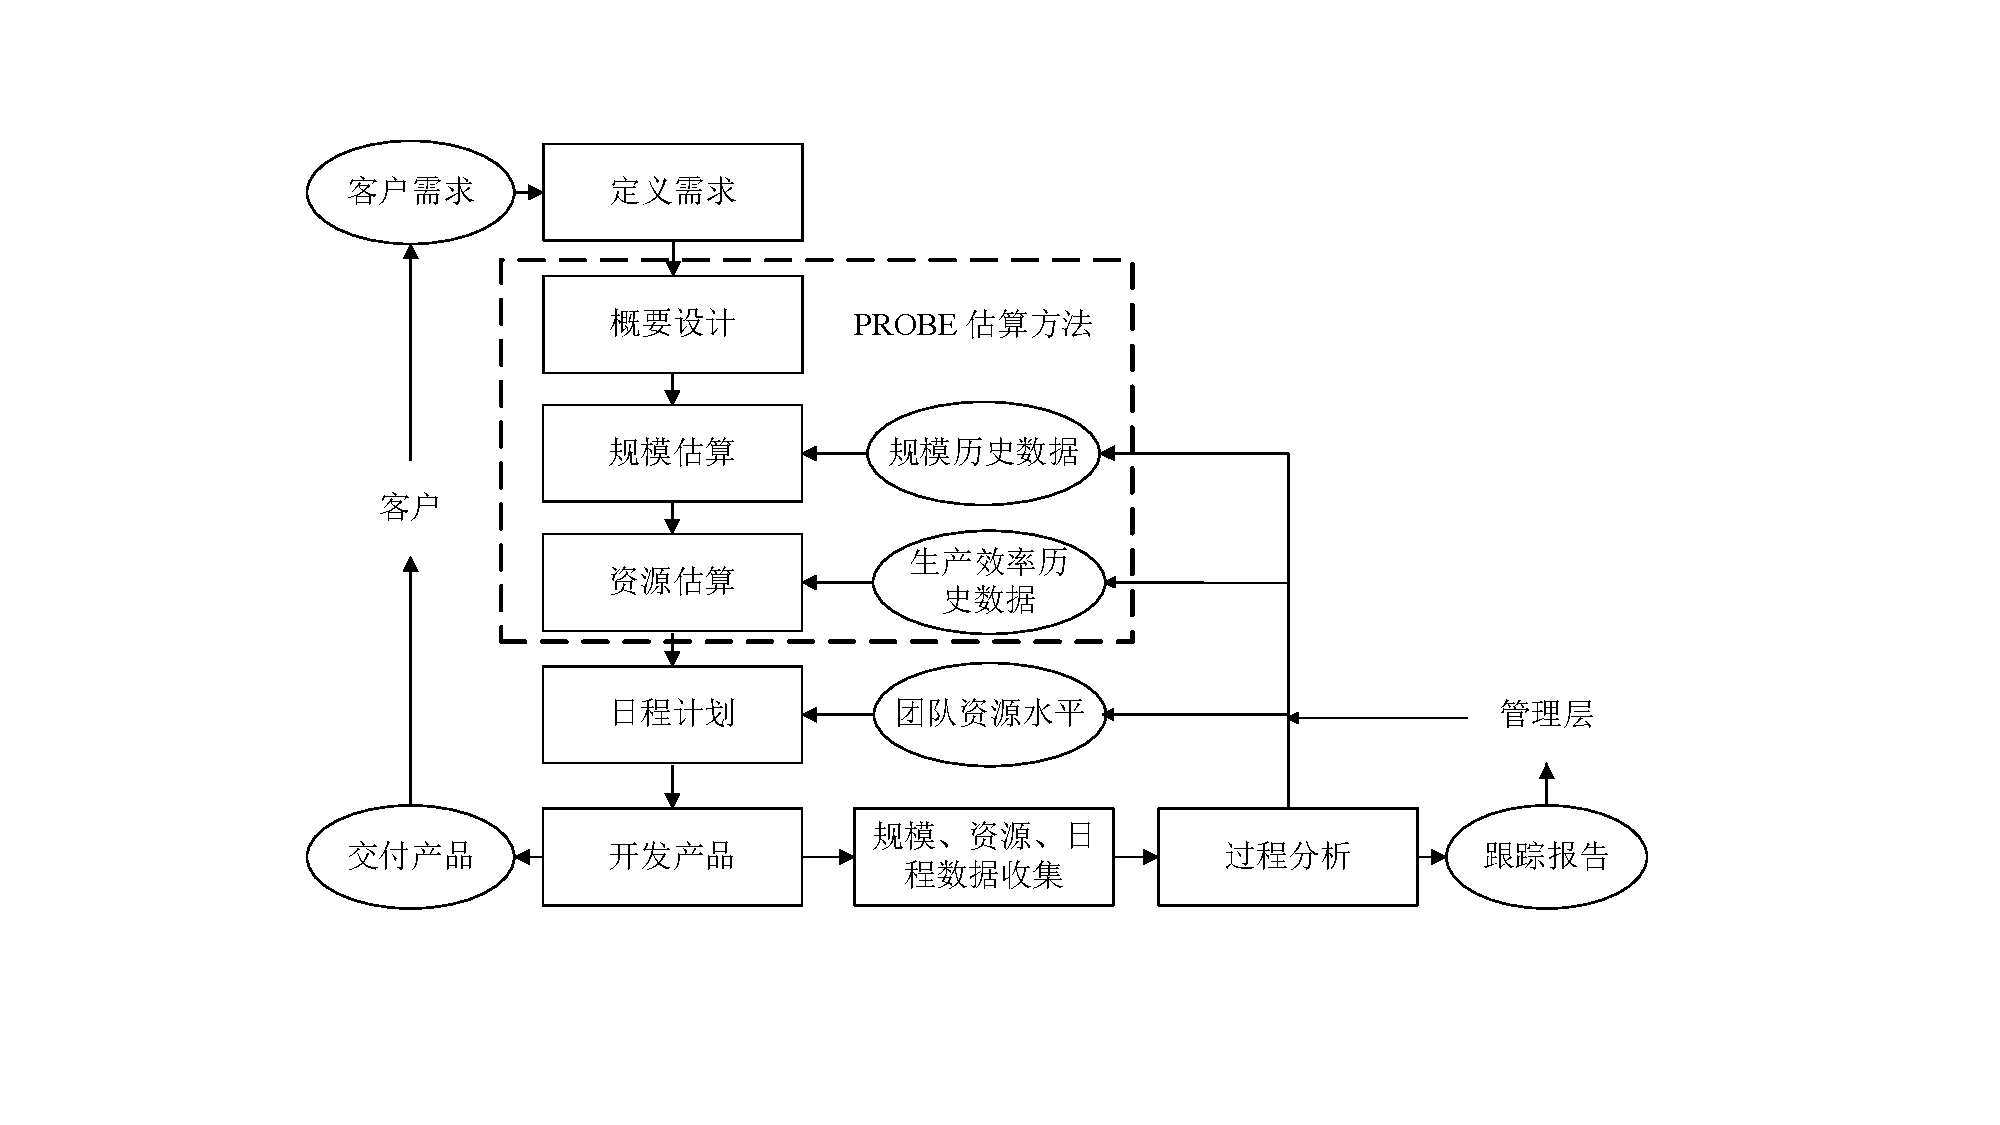
\includegraphics[width=0.8\textwidth]{通用计划框架.pdf}
\end{figure}
\end{solution}



\begin{problem}[2013、2015A、2018]
谈谈你对项目估算的认识,并简要解释应用PROBE方法估算的优缺点。
\end{problem}

\begin{solution}
规模估算往往可以依据历史数据来完成,其原因在于规模估算结果的偏差产生原因相对客观,偏差可以用以修正新的估算结果。

时间估算的偏差产生原因更加复杂,一方面和规模有关,另外一方面,跟人的主观能动性有关,因此,时间估算偏 差的原因可能估算结果本身,这使得历史数据中时间偏差可参考价值不大。

从上述讨论可以得出,对于估算来说,本质上是一种猜测,追求的目标应该是一致性以及 估算结果的使用者对估算结果的信心。

PROBE方法通过定义的估算过程和数据收集以及使用的框架,使得估算结果可以尽可能一致,从而使得一些统计方法可以用来调整估算结果,增强用户对估算结果的信心。

但是这种估算方法非常依赖高质量的历史数据,一旦数据不完整或者缺失,就可能导致估算结果有显著偏差。
\end{solution}



\begin{problem}[2023]
软件项目规模估算的基本要点有哪些?
\end{problem}

\begin{solution}
\vspace{-0.8em}
\begin{multicols}{2}
    \begin{itemize}
        \item 尽可能划分详细一些:估算多个部件的时候,总的误差会比各个部件的误差的总和小
        \item 建立对结果的信心
        \item 依赖数据
        \item 估算要的是过程,而非结果,估算的过程是相关干系人达成一致共识的过程
    \end{itemize}
\end{multicols}
\vspace{-1em}
\end{solution}



\begin{problem}[2018、2020]
请描述一下 PROBE 方法的基本原理和过程,并解释在应用 PROBE A 方法估算时间的时候,为什么不用历史数据中的生产效率数据。
\end{problem}

\begin{solution}
估算的原理:
\begin{itemize}
    \item 设立合理的代理作为精确度量和早期规划需要的度量之间的桥梁
    \item 相对大小,而非绝对大小
\end{itemize}

估算的过程:

\begin{figure}[H]
	\centering
	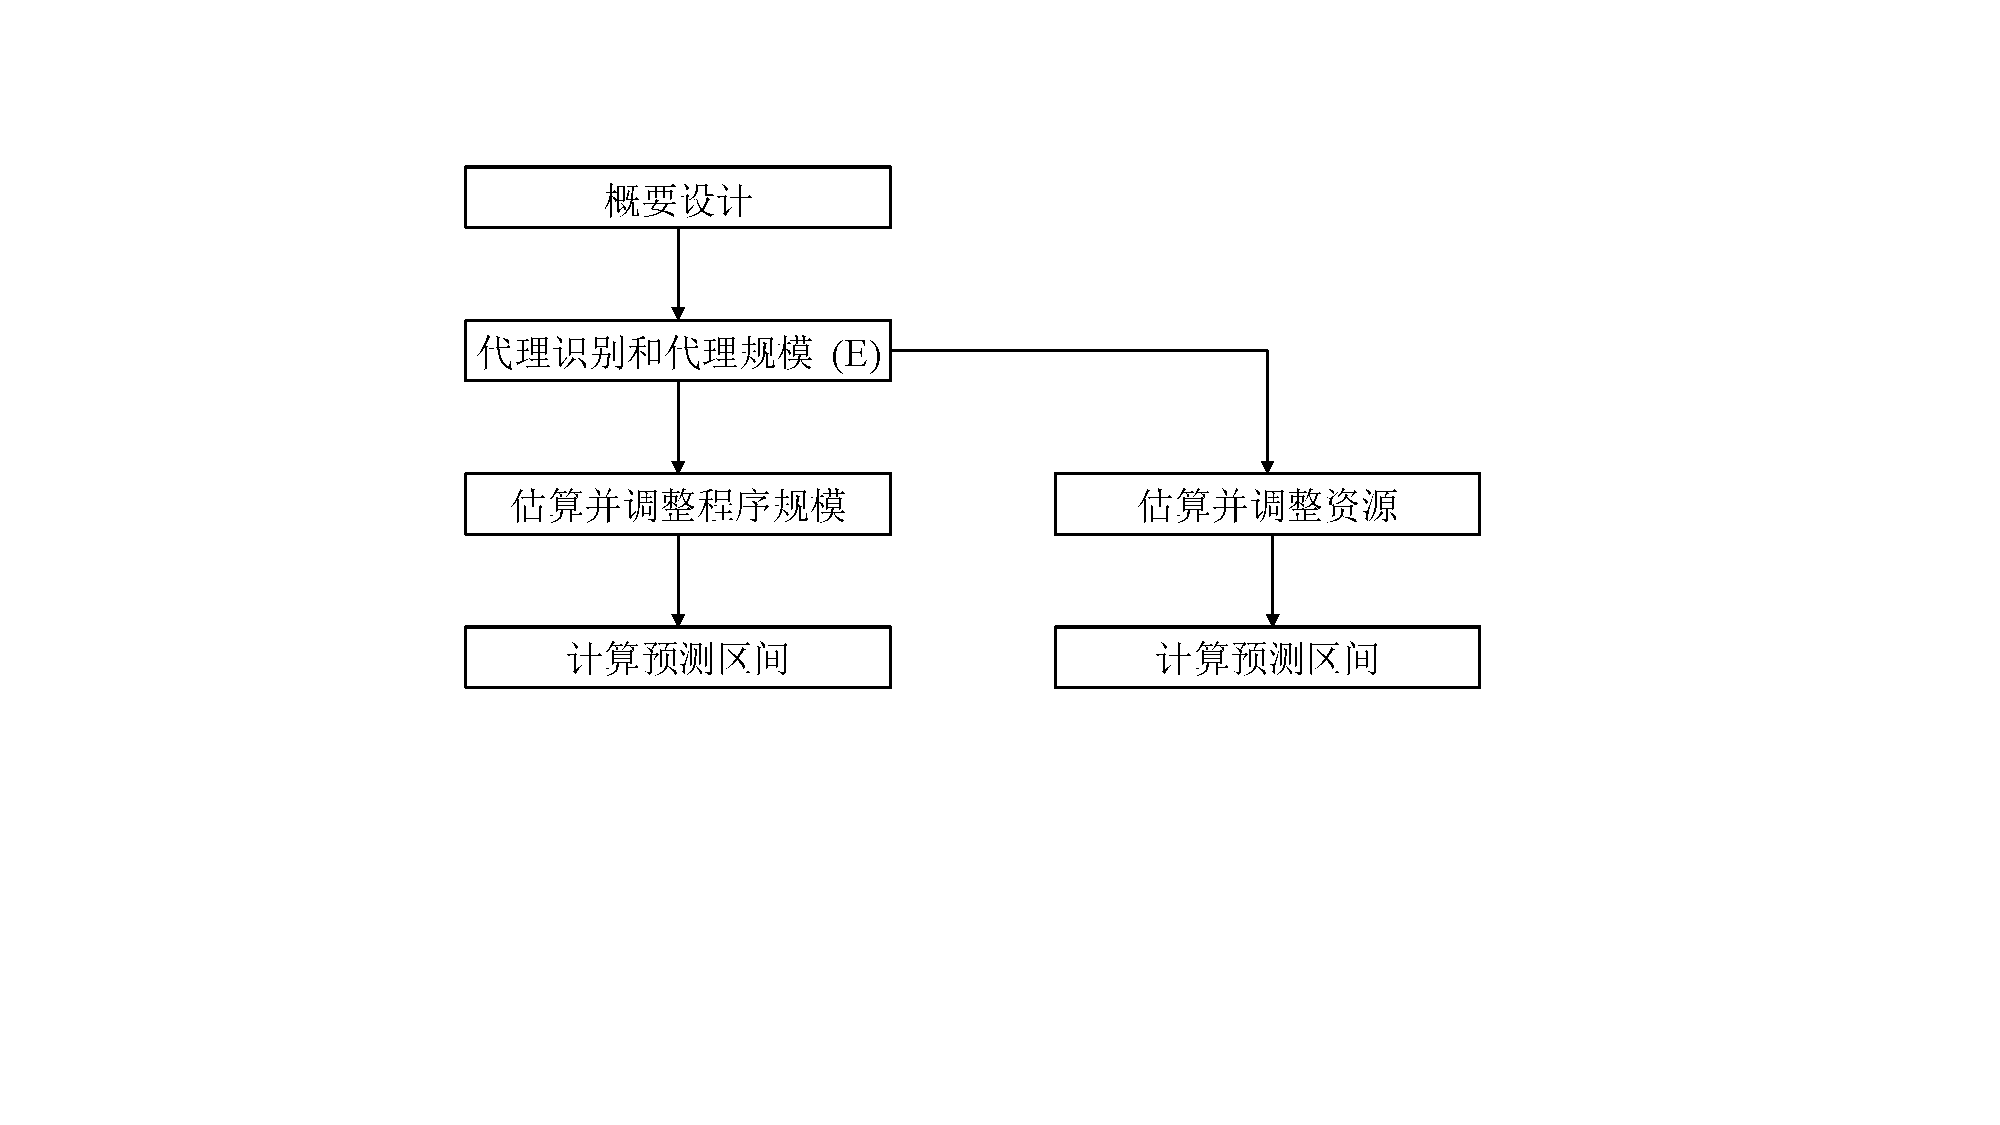
\includegraphics[width=0.6\textwidth]{估算过程.pdf}
\end{figure}

不适用生产效率的理由:在估算资源需求(例如人时)的时候,生产效率一般在分母上,考虑到个体软件工程师生产效率波动,易导致的估算偏差范围变大。
\end{solution}



\begin{problem}[2020]
请描述PROBE ABCD方法在估算规模的时候,对历史数据的质量有什么要求? 
\end{problem}

\begin{solution}
规模估算:
\vspace{-0.5em}
\begin{spacing}{1.2}
    \centering
    \begin{longtable}{|m{2.3cm}<{\centering}|m{3cm}|m{4cm}|m{2.3cm}<{\centering}|}
        \hline
        \textbf{PROBE方法} & \multicolumn{1}{c|}{\textbf{数据要求}} & \multicolumn{1}{c|}{\textbf{数据质量要求}}                                                 & \multicolumn{1}{c|}{\textbf{计算方法}} \\ \hline
        A & 3组或者3组以上代理规模(E)与实际程序规模 &
        \vspace{-1em}
        \begin{enumerate}[label=\arabic*.,leftmargin=1.2em,itemsep=-2pt]
            \item $r\geq 0.7$
            \item $s\leq 0.05$
            \item $\beta 0 \leq$ 估算结果的25\%
            \item $0.5\leq \beta 1 \leq 2$    
        \vspace{-1.3em}
        \end{enumerate}
        & 略 \\ \hline
        B & 3组或者3组以上计划程序规模与实际程序规模 &
        \vspace{-1em}
        \begin{enumerate}[label=\arabic*.,leftmargin=1.2em,itemsep=-2pt]
            \item $r\geq 0.7$
            \item $s\leq 0.05$
            \item $\beta 0 \leq$ 估算结果的25\%
            \item $0.5\leq \beta 1 \leq 2$    
        \vspace{-1.3em}
        \end{enumerate}
        & 略 \\ \hline
        C & 有历史数据 & 无 & 按比例调整 \\ \hline
        D & 没有历史数据 & 无 & 猜测 \\ \hline
    \end{longtable}
	\end{spacing}
\vspace{-1em}

时间估算:
\vspace{-0.5em}
\begin{spacing}{1.2}
    \centering
    \begin{longtable}{|m{2.3cm}<{\centering}|m{3cm}|m{5.7cm}|m{2.3cm}<{\centering}|}
        \hline
        \textbf{PROBE方法} & \multicolumn{1}{c|}{\textbf{数据要求}} & \multicolumn{1}{c|}{\textbf{数据质量要求}}                                                 & \multicolumn{1}{c|}{\textbf{计算方法}} \\ \hline
        A & 3组或者3组以上代理规模(E)与实际程序规模 &
        \vspace{-1em}
        \begin{enumerate}[label=\arabic*.,leftmargin=1.2em,itemsep=-2pt]
            \item $r\geq 0.7$
            \item $s\leq 0.05$
            \item $\beta 0$显著小于估算结果
            \item $\beta 1 \leq 0.5\times$(历史生产效率的倒数)
        \vspace{-1.3em}
        \end{enumerate}
        & 略 \\ \hline
        B & 3组或者3组以上计划程序规模与实际程序规模 &
        \vspace{-1em}
        \begin{enumerate}[label=\arabic*.,leftmargin=1.2em,itemsep=-2pt]
            \item $r\geq 0.7$
            \item $s\leq 0.05$
            \item $\beta 0$显著小于估算结果
            \item $\beta 1 \leq 0.5\times$(历史生产效率的倒数)
        \vspace{-1.3em}
        \end{enumerate}
        & 略 \\ \hline
        C & 有历史数据 & 无 & 按比例调整 \\ \hline
        D & 没有历史数据 & 无 & 猜测 \\ \hline
    \end{longtable}
	\end{spacing}
\vspace{-1em}
\end{solution}



\begin{problem}[2013、2021]
基于Yield指标构建缺陷预测模型,并列举该模型的可能改进方案
\end{problem}

\begin{solution}
总体思想:利用回归技术预测软件开发过程中各阶段的Inject Rate(缺陷注入率)和Yield(缺陷消除率)

Yield指标只能用来估算,不可以用来度量。结合Yield指标和下图,只需要知道如下指标就可以基于Yield指标构建一个基本的缺陷预测模型:
\vspace{-0.8em}
\begin{multicols}{2}
    \begin{itemize}
        \item 注入阶段注入多少缺陷
        \item 缺陷注入的密度(需求每一页注入多少缺陷)
        \item 缺陷注入的速度(每小时注入多少缺陷)
        \item 消除阶段的缺陷注入密度和速度。
        \item 历史数据中的软件规模、文档规模、开发人员规模
    \end{itemize}
\end{multicols}
\vspace{-1em}

步骤:
\vspace{-0.8em}
\begin{multicols}{2}
    \begin{enumerate}[label=\arabic*.]
        \item 确定纳入影响因子的数据以及数据度量方法
        \item 从系统历史库中收集历史数据,并进行整理
        \item 依照回归技术进行计算
        \item 在项目进行过程中不断收集数据,与预测数据进行比较,调整回归参数
        \item 项目过程中依据实际数据与预测数据的误差进行风险的预防、识别和控制
    \end{enumerate}
\end{multicols}
\vspace{-1em}

下图第一个消除步骤是需求评审,第二个消除步骤是设计评审,第三个消除步骤是测试评审

\begin{figure}[H]
    \vspace{-0.5em}
	\centering
	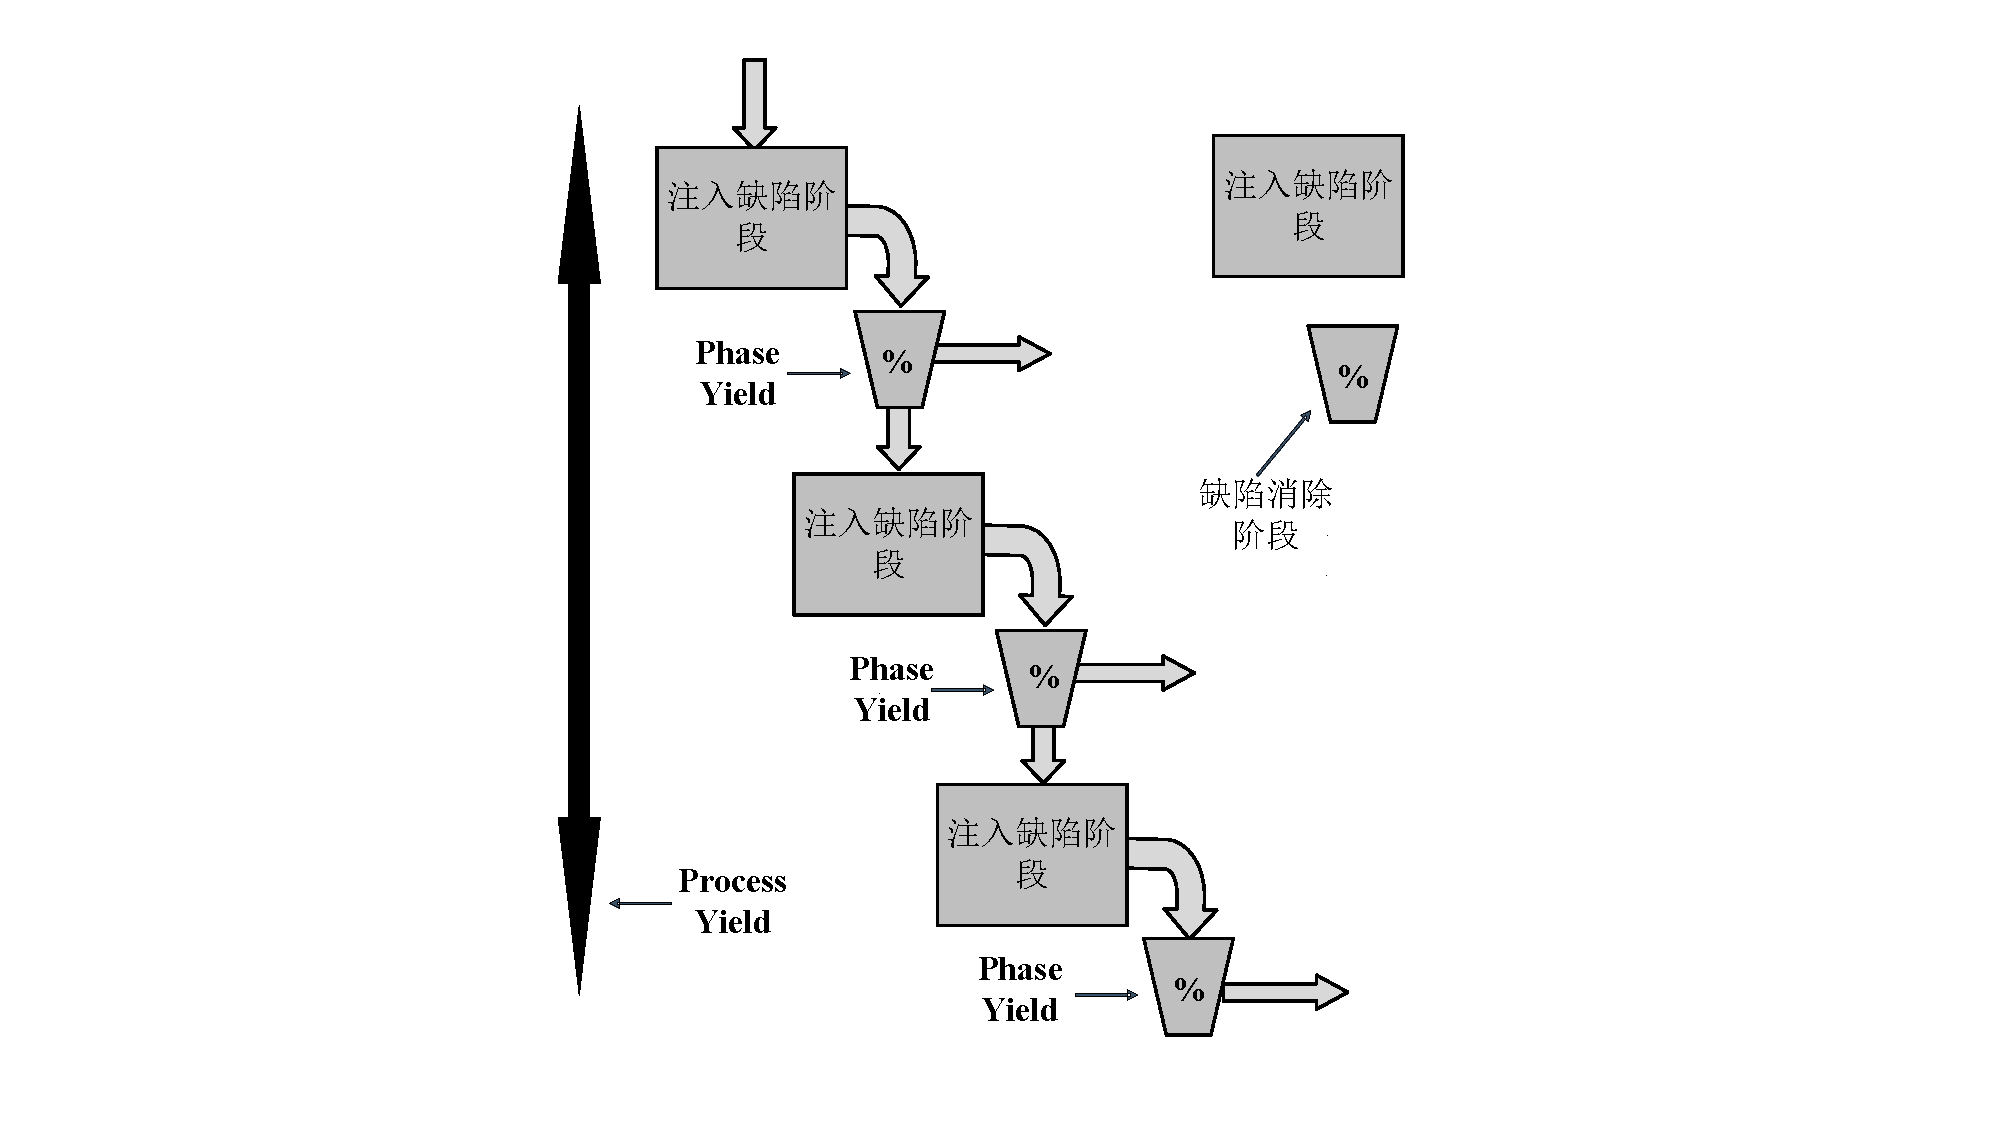
\includegraphics[width=0.42\textwidth]{缺陷在开发过程中注入和消除的示意图.pdf}
    \vspace{-1em}
\end{figure}

改进方案:
\begin{itemize}
    \item 结果受限于历史数据在简单性、可理解性、稳定性、可度量性、相关性等方法的质量。因此,维护历史数据。
    \item 影响因子的选择上面不仅仅需要有关软件规模的数据,还需要有关开发过程、开发文档、开发人员等方面的数据,并且需要将数据可度量化。
    \item 反馈模型。即在开发过程中随着实际数据的产生,将这些数据作为输入变量放入模型中以调整回归参数。
    \item (重要)可能的改进是假设注入水平和消除水平都符合正态分布,计算均值和标准差,因此,可以用蒙特卡罗方法模拟结果。
\end{itemize}
\end{solution}



\begin{problem}[2016]
DevOps的三个步骤
\end{problem}

\begin{solution}
\begin{enumerate}[label=\arabic*.]
    \item 实现开发到运维的工作快速地从左向右流动。
    \item 从右向左的每个阶段,采用持续、快速的工作反馈机制。
    \item 建立具有创意和高可信度的企业文化,支持动态的、严格的、科学的实验。
\end{enumerate}
\end{solution}



\begin{problem}
DevOps的特点,为什么流行?
\end{problem}

\begin{solution}
DevOps 以敏捷项目管理技术和微服务支持为中心,通过基于版本控制标准的自动化来处理整个软件开发生命 周期。Git 是 DevOps 中最流行的版本控制解决方案,DevOps 还包括管理软件生命周期、自动化代码测试、 容器编排、云托管和数据分析的 CI/CD 要求 。

DevOps 的好处:
\begin{itemize}
    \item 敏捷团队项目管理:增强网站和移动应用软件开发的管理。
    \item 软件开发过程的优化:通过持续集成和持续交付 (CI/CD) 功能实现。借助 CI/CD,公司可以通过代码更改 快速推出新的软件功能,从而将新的创新推向市场。使用自动版本控制系统和容器简化了 Web 服务器代码或应用程序脚本的升级。
    \item 促进协作:Git 允许开发人员在具有订单项回滚能力的团队中进行协作。
    \item 通过自动化提高效率:CI/CD 通过企业编程工具、IDE 和第三方实用程序支持自动化代码测试。DevOps 使采用它来管理软件开发生命周期的公司能够更好地自动化数据中心流程、Web 服务器配置、数据库管 理、知识共享、部署调度和商业智能。
\end{itemize}
\end{solution}



\begin{problem}[2021]
解释至少5个DevOps技术、实践、方法
\end{problem}

\begin{solution}
典型软件过程和实践:DevOps
\vspace{-0.8em}
\begin{multicols}{2}
    \begin{itemize}
        \item 开发运维一体化
        \item 方法论的基础是软件敏捷开发、精益思想和看板 KanBan 方法
        \item 以领域驱动设计为指导的微服务架构方式
        \item 大量虚拟化技术的使用
        \item 一切皆服务 XaaS 的理念指导
        \item 构建了强大的工具链,支持高水平自动化
    \end{itemize}
\end{multicols}
\vspace{-1em}

可遵循的DevOps最佳实践:
\vspace{-0.8em}
\begin{multicols}{2}
    \begin{enumerate}[label=\arabic*.]
        \item 培养协作和无责沟通的文化
        \item 采用持续集成和交付(CI/CD)
        \item 设置自动化测试
        \item 关注可观察性并找到正确的指标
        \item 使用自动化避免手动工作
        \item 在开发生命周期的早期加入安全性
        \item 从事件中学习并围绕它们构建流程
        \item 首先关注概念,然后找到合适的工具
        \item 采用基础设施即代码(IaC)并推动自助式基础设施模型
    \end{enumerate}
\end{multicols}
\vspace{-1em}
\end{solution}



\begin{problem}[2013、2015、2018]
请解释A/FR,PQI的计算方式,并且解释这两个指标有什么用途?
\end{problem}


\begin{solution}
A/FR (Appraisal to Failure Ratio),质检失效比
\vspace{-0.8em}
\begin{multicols}{2}
    \begin{itemize}
        \item A/FR $=$ PSP质检成本 / PSP失效成本
        \item 质检成本 $=$ 设计评审时间 $+$ 代码评审时间
        \item 失效成本 $=$ 编译时间 $+$ 单元测试时间
    \end{itemize}
\end{multicols}
\vspace{-1em}

用途:理论上,A/FR值越大,意味着质量越高,但A/FR值过大说明评审过多,则开发效率低下,因此PSP中A/FR期望值为2.0

PQI(Process Quality Index, 过程质量指标)为5个数据的乘积(以基准值作为1,最后结果越接近1,质量越高)
\begin{itemize}
    \item 设计质量:设计时间应该大于编码时间,$\min(\frac{\scriptsize{\mbox{设计时间}}}{\scriptsize{\mbox{编码时间}}}, 1)$
    \item 设计评审质量:设计评审的时间应该大于设计时间的50\%,$\min(2 \times \frac{\scriptsize{\mbox{设计评审时间}}}{\scriptsize{\mbox{设计时间}}}, 1)$
    \item 代码评审质量:代码评审时间应该大于编码时间的50\%,$\min(2 \times \frac{\scriptsize{\mbox{代码评审时间}}}{\scriptsize{\mbox{编码时间}}}, 1)$
    \item 代码质量:代码的编译缺陷密度应当小于10个/千行,$\min(\frac{20}{\scriptsize{\mbox{编译缺陷密度}} + 10}, 1)$
    \item 程序质量:代码的单元测试缺陷密度应当小于5个/千行,$\min(\frac{10}{\scriptsize{\mbox{单元测试缺陷密度}} + 5}, 1)$
\end{itemize}

用途:
\vspace{-0.8em}
\begin{multicols}{3}
    \begin{itemize}
        \item 判断模块开发质量
        \item 规划质量活动计划
        \item 过程改进
    \end{itemize}
\end{multicols}
\vspace{-1em}
\end{solution}


\begin{problem}[2015A]
请结合A/FR、PQI、Review Rate、DRL、Yield尽可能具体描述一个软件项目应该如何从多方面来确保开发的高质量?
\end{problem}

\begin{solution}
这些指标既是开发过程中质量管理的一些参考指标,同时也体现在计划安排中应该注意的质量元素。具体如下:
\begin{itemize}
    \item 在项目计划过程中应该安排确保高质量开发结果的活动,例如,按照A/FR、PQI等指标的要求,安排对各类产物(文档和代码)的个人评审和小组评审
    \item 这些评审活动应该满足一定的要求,特别体现在时间方面。例如,评审时间应该多于测试时间的两倍以上(A/FR);评审时间应该是相应开放时间的50\%以上(PQI);评审速度要求(Review Rate)等
    \item 充分借鉴质量指标所体现的开发质量状况,尽早制订相应的质量补救措施。例如,PQI所体现的缺陷密度、所有上述指标的参考值等等。一旦超标,往往意味着质量方面有偏差,应当及时补救
    \item 利用Yield等指标,构建质量预测模型,更加积极(Proactive)地判定和控制开发质量
    \item 依据PQI和Yield指标所体现的信息,通过过程改进来提升开发质量
\end{itemize}
\end{solution}



\begin{problem}[2013、2015A]
如果对质量的追求是无止境的,在不考虑资源和成本的前提下,有哪些可能有效的策略?
\end{problem}

\begin{solution}
\vspace{-0.8em}
\begin{multicols}{2}
    \begin{enumerate}[label=\arabic*.]
        \item 重视测试,并且将测试过程文档化并且稳定化
        \item 重视小组评审,同样定义评审过程,并且使得评审过程的performance稳定化
        \item 重视个人评审,提升评审者技能
        \item 重视设计
        \item 开展设计验证
    \end{enumerate}
\end{multicols}
\vspace{-1em}
\end{solution}



\begin{problem}[2015]
请给出需求开发的完整过程,并且解释客户需求和产品需求的各自含义以及在需求开发过程中该如 何体现客户需求和产品需求?
\end{problem}

\begin{solution}
需求获取、需求汇总、需求验证、需求文档制作

客户需求描述的是客户的期望。往往表现为,客户在实际工作中碰到了一些具体问题,希望通过某个东⻄来帮忙解决这些问题。客户的这种解决问题的愿望,往往就表述为客户需求。比如,客户希望有一种快速进行数据计算的工具帮助他/她完成繁琐的计算工作。这就是一个客户需求。客户需求可能很简单,也可能很复杂;可能很清晰,也可能很模糊。这就需要开发团队与客户一起进行交流、协商,从而弄清客户的真正意图。

产品需求描述的是开发团队所提供的解决方案。即针对上述的客户需求,开发团队设计出一个可以帮助客户解决工作当中碰到的问题的方案。
\end{solution}



\begin{problem}[2015B]
请解释在质量保障活动中的V\&V分别是什么含义?两者之间的关系是什么?
\end{problem}

\begin{solution}
验证是目的是确保选定的工作产品与事先指定给该工作产品的需求(即产品需求或产品组件需求)一致

确认的目的则是确保开发完成的产品或者产品组件在即将要使用该产品或者产品组件的环境中工作正确,关注的是客户需求的满足

验证和确认又是相互依存、关系紧密的两个活动。二者都是为了提升最终产品的质量而采取的措施
\begin{itemize}
    \item 验证活动的依据来源于确认的目标,即产品组件需求必须与客户需求一致
    \item 验证活动为确认活动提供了前提条件,在完成产品需求和产品组件需求之前,考虑客户需求是否满足是没有意义的
\end{itemize}
\end{solution}



\begin{problem}[2013、2014、2015A、2015B、2016]
如何制定一份让人无法拒绝的计划,请描述基本步骤和一些注意事项。
\end{problem}

\begin{solution}
\begin{itemize}
    \item 制定任务计划和日程计划:前者描述项目所有的任务清单,任务之间的先后顺序、以及每个任务所需时间资源,后者描述了各个任务在日程上的安排,哪天开始哪天结束
    \item 制定资源计划
    \item 这种日程计划的关键是必须用正推的方式来制订项目计划。一个典型的项目计划框架如下图
    \item 在这个过程中,除了概要设计和资源估算之外,其他环节尽可能自动化完成。充分参考历史数据进行估算
\end{itemize}

\begin{figure}[H]
    \vspace{-0.7em}
	\centering
	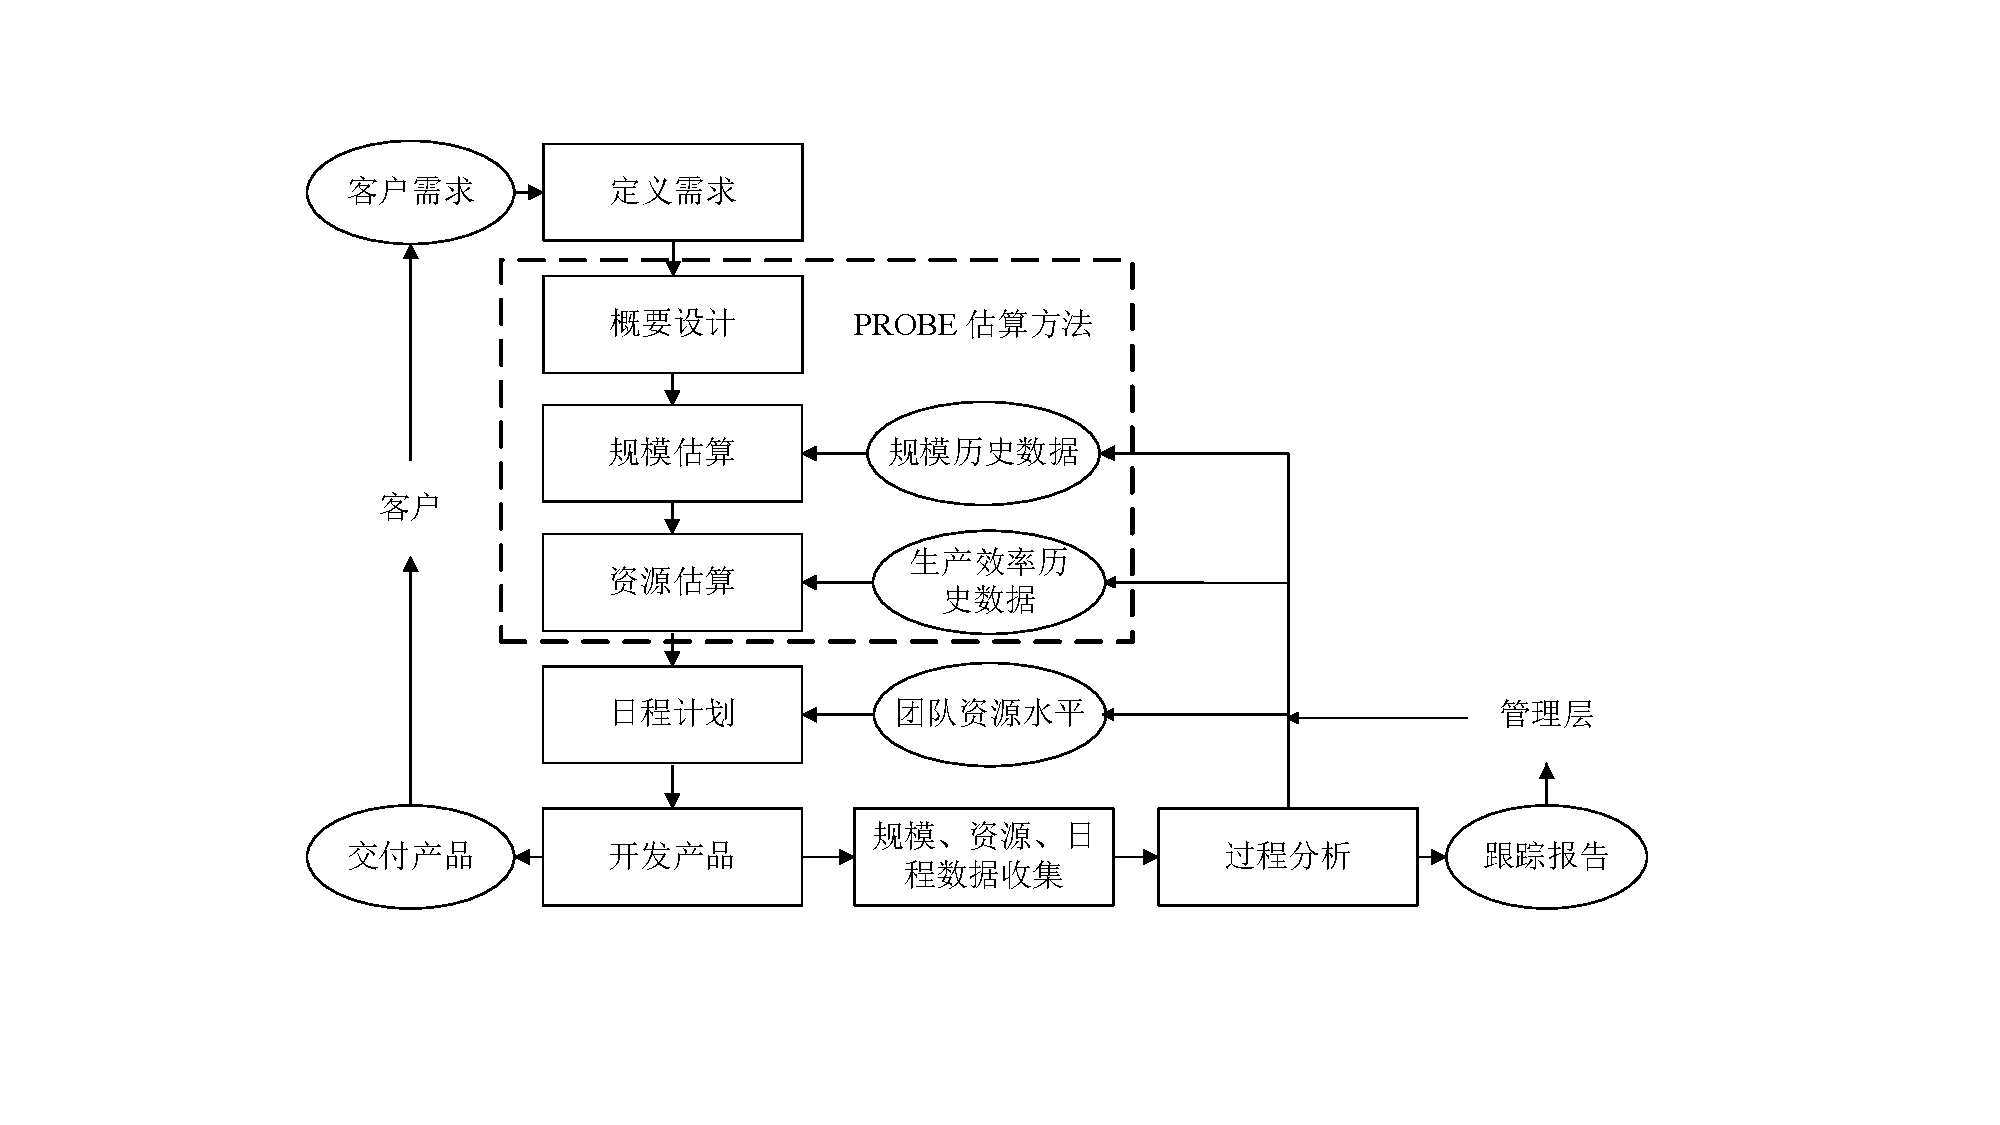
\includegraphics[width=0.7\textwidth]{通用计划框架.pdf}
    \vspace{-1em}
\end{figure}
\end{solution}



\begin{problem}[2023]
挣值管理有三种实现方式,分别是简单、中级和高级。分别阐述上述三种方式的基本要点。
\end{problem}

\begin{solution}
\textbf{简单实现}:仅仅关注进度信息
\begin{itemize}
    \item 实现方式
    \begin{itemize}
        \item 首先需要建立WBS,定义工作范围
        \item 其次为WBS中每一项工作定义一个计划价值(PV, Planned Value)
        \item 最后按照一定的规则将某一数值赋给已经完成的工作或者正在进行的工作,该值成为挣值(EV, Earned Value)
    \end{itemize}
    \item 常用规则
    \begin{itemize}
        \item 0-100原则:只有当某项任务完成时,该任务的PV值将转化成EV值
        \item 50-50原则:只需要开始某项任务,即可以赋原PV值的50\%作为EV值,完成时,再加上另外的50\%
        \item 实际完成的工作所需成本AC不对EV值产生任何影响
    \end{itemize}
\end{itemize}

\textbf{中级实现}
\begin{itemize}
    \item 在简单实现的基础上,加入日程偏差的计算,加入了成本线(AC)
    \item 典型计算方式有
    \vspace{-0.8em}
    \begin{multicols}{2}
        \begin{itemize}
            \item 日程偏差SV = EV $-$ PV
            \item 日程偏差指数SPI = EV/PV;
        \end{itemize}
    \end{multicols}
    \vspace{-1em}
\end{itemize}

\textbf{高级实现}:添加预测线(BAC),当任务足够多的时候,我们就可以让预测线尽可能平直,同时我们延伸挣值(EV),找到与预测线(BAC)的交点,我们就可以明确项目的落后时间

\begin{figure}[H]
    \vspace{-0.5em}
	\centering
	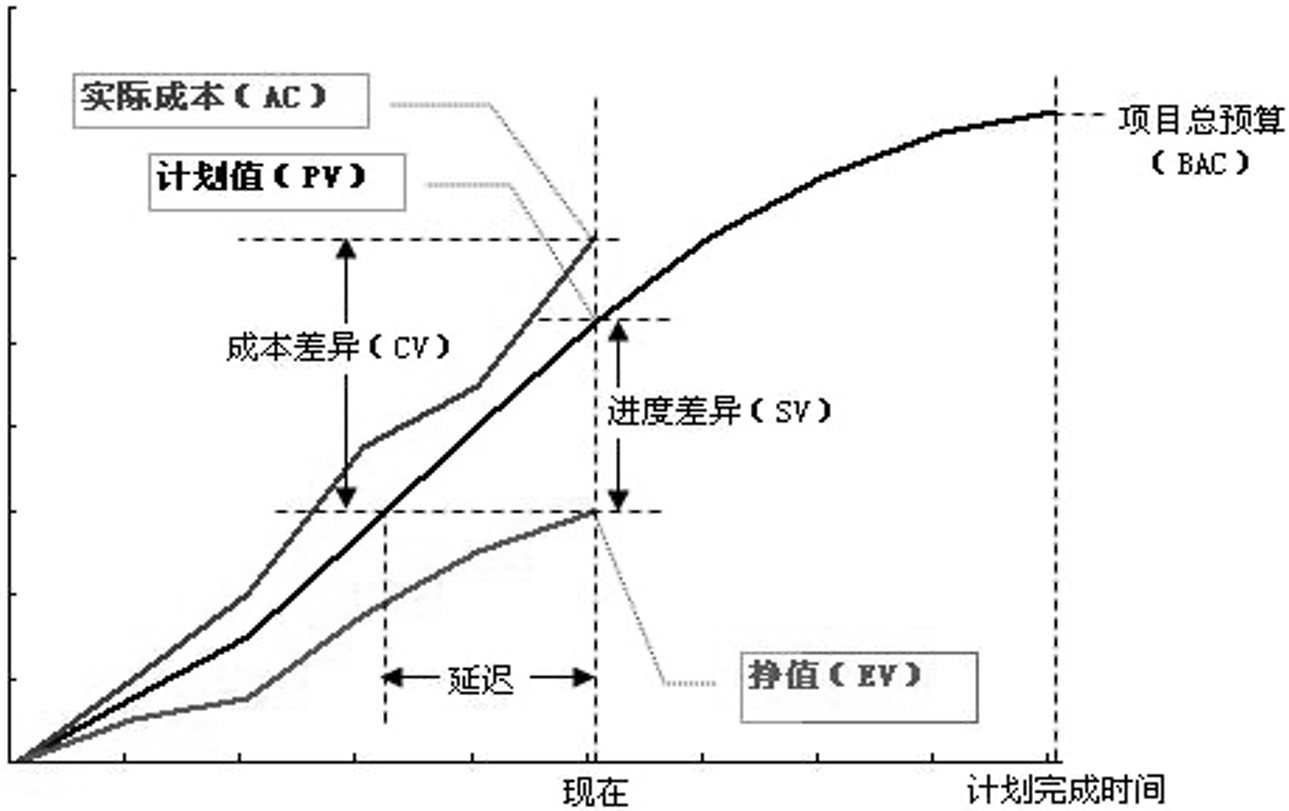
\includegraphics[width=0.6\textwidth]{挣值管理图解.png}
    \vspace{-1em}
\end{figure}

\begin{itemize}
    \item 上面的线是为了获取这些挣值付出的实际代价,这个线和挣值之间的差异是成本差异
    \item 中间的线是预算(每天需要完成多少挣值)BAC,理想情况下是一条直线
    \item 下面的线是挣值(实际的进展情况)EV,和owner value有关,对应plan value
    \item 实际获取挣值和预计获取挣值的差异是进度差异
    \item 挣值管理会带来什么好处?可以很好的适应项目的动态变化
\end{itemize}
\end{solution}



\begin{problem}[2013、2014、2015、2016、2020]
请结合软件开发特点介绍软件项目管理中自主型团队的必要性

自主团队有哪些特点?为什么说这样的团队可以满足软件开发对团队的要求

请结合软件开发的特点介绍软件项目管理中自主型团队的必要性以及自主团队应该具备的特征?
\end{problem}

\begin{solution}
软件开发是一项既复杂又富有创造性的知识工作

软件开发是一种智力劳动:处理和讨论极其抽象的概念、把不同的部分(不可见)整合成一个可以工作的系统

软件开发是一种智力活动,开发者是智力劳动者,而对于智力劳动者而言,管理的第一准则就是智力劳动者不能被管理,只能实现自我管理:
\vspace{-0.8em}
\begin{multicols}{2}
    \begin{itemize}
        \item 处理和讨论非常抽象的概念
        \item 把不同的部分整合成一个可以工作的正确的系统
        \item 全身心地参与
        \item 努力做出卓越的工作
    \end{itemize}
\end{multicols}
\vspace{-1em}

自主团队具备如下的特点:
\vspace{-0.8em}
\begin{multicols}{2}
    \begin{itemize}
        \item 自行定义项目的目标
        \item 自行决定团队组成形式以及成员的角色
        \item 自行决定项目的开发策略
        \item 自行定义项目的开发过程
        \item 自行制定项目的开发计划
        \item 自行度量、管理和控制项目工作
    \end{itemize}
\end{multicols}
\vspace{-1em}
\end{solution}



\begin{problem}[2023]
结合“软件开发作为一种知识工作,需要领导者而不是一般的经理”,阐述知识工作领导者应该具备的品质或者特点(至少三项)。
\end{problem}

\begin{solution}
\begin{enumerate}[label=\arabic*.]
    \item 善于倾听团队成员的想法,并加以分析和改进
    \item 善于通过询问来诱导团队成员向着正确的方向前进
    \item 善于通过激励以及设定挑战目标等方式吸引团队成员努力表现
    \item 当出现不一致意见的时候,领导者则善于提供各种沟通方式,促成团队达成一致意见
    \item 培养团队成员技能
    \item 鼓励建立起合理的授权机制
    \item 通过挑战建立目标,确定团队努力方向
\end{enumerate}
\end{solution}



\begin{problem}[2021]
列出TSP角色并解释其中5个的职责
\end{problem}

\begin{solution}
\vspace{-0.5em}
\begin{spacing}{1.2}
    \centering
    \begin{longtable}{|m{1.5cm}<{\centering}|m{4.2cm}|m{4.2cm}|m{4.2cm}|}
        \hline
        \textbf{角色} & \multicolumn{1}{c|}{\textbf{介绍}} & \multicolumn{1}{c|}{\textbf{典型技能}} & \multicolumn{1}{c|}{\textbf{工作内容}} \\ \hline
        \textbf{项目组长} & 
        项目组长的目标和衡量指标
        \begin{itemize}[leftmargin=1.3em]
            \item 建设和维持高效率的团队
            \item 激励团队成员积极工作
            \item 合理处理团队成员的问题
            \item 向管理层提供项目进度相关的完整信息
            \item 充当合格的会议组织者和协调者
            \vspace{-1.3em}
        \end{itemize} &
        \vspace{-1.1em}
        \begin{itemize}[leftmargin=1.3em]
            \item 你是天生的领导者
            \item 你有能力识别问题的关键并且做出客观的决策
            \item 你不介意偶尔充当“恶人”
            \item 你尊敬你的团队成员
            \vspace{-1.3em}
        \end{itemize} &
        \vspace{-1.1em}
        \begin{enumerate}[label=\arabic*.,leftmargin=1.5em]
            \item 激励团队成员努力工作
            \item 主持项目周例会
            \item 每周汇报项目状态
            \item 分配工作任务
            \item 维护项目资料
            \item 组织项目总结
            \vspace{-1.3em}
        \end{enumerate} \\ \hline
        \textbf{计划经理} & 
        \vspace{-1.1em}
        \begin{itemize}[leftmargin=1.3em]
            \item 开发完整的、准确的团队计划和个人计划
            \item 每周准确的报告项目小组状态
            \vspace{-1.3em}
        \end{itemize} &
        \vspace{-1.1em}
        \begin{itemize}[leftmargin=1.3em]
            \item 最为重要的一点是,你做事有条理和逻辑
            \item 你对于过程数据非常感兴趣,期待通过每周输入的数据来了解项目当前状况
            \item 你认为计划非常重要,也愿意要求团队成员跟踪和度量他们的工作
            \vspace{-1.3em}
        \end{itemize} &
        \vspace{-1.1em}
        \begin{enumerate}[label=\arabic*.,leftmargin=1.5em]
            \item 带领项目小组开发项目计划
            \item 带领项目小组平衡计划
            \item 跟踪项目进度
            \item 参与项目总结
            \vspace{-1.3em}
        \end{enumerate} \\ \hline
        \textbf{开发经理} & 
        \vspace{-1.1em}
        \begin{itemize}[leftmargin=1.3em]
            \item 开发优秀的软件产品
            \item 充分利用团队成员的技能
            \vspace{-1.3em}
        \end{itemize} &
        \vspace{-1.1em}
        \begin{itemize}[leftmargin=1.3em]
            \item 你喜欢创造事物
            \item 你愿意成为软件工程师,并且喜欢带领团队开展设计和开发工作
            \item 你具备足够的背景可以胜任设计师的工作,并且可以领导设计团队开展工作
            \item 你熟悉主流的设计工具
            \item 你愿意倾听和接受其他人的设计思想
            \vspace{-1.3em}
        \end{itemize} &
        带领团队
        \vspace{0.2em}
        \begin{enumerate}[label=\arabic*.,leftmargin=2.1em]
            \item 制定开发策略
            \item 开展产品规模估算和所需时间资源的估算
            \item 开发需求规格说明
            \item 开发高层设计
            \item 开发设计规格说明
            \item 实现软件产品
            \item 开展集成测试和系统测试
            \item 开发用户支持文档
        \end{enumerate}
        \vspace{0.3em}
        \begin{enumerate}[label=9.,leftmargin=1.5em]
            \item 参与项目总结
            \vspace{-1.3em}
        \end{enumerate} \\ \hline
        \textbf{质量经理} & 
        \vspace{-1.1em}
        \begin{itemize}[leftmargin=1.3em]
            \item 项目团队严格按照质量计划开展工作,开发出高质量的软件产品
            \item 所有的小组评审工作都正常开展,并且都形成了评审报告
            \vspace{-1.3em}
        \end{itemize} &
        \vspace{-1.1em}
        \begin{itemize}[leftmargin=1.3em]
            \item 你关注软件产品的质量
            \item 你有评审方面的经验,熟悉各种评审方法
            \item 你有协调组织有效评审的能力
            \vspace{-1.3em}
        \end{itemize} &
        \vspace{-1.1em}
        \begin{enumerate}[label=\arabic*.,leftmargin=1.5em]
            \item 带领团队开发和跟踪质量计划
            \item 向项目组长警示质量问题
            \item 软件产品提交配置管理之前,对其进行评审,以消除质量问题
            \item 项目小组评审的组织者和协调者
            \item 参与项目总结
            \vspace{-1.3em}
        \end{enumerate} \\ \hline
        \textbf{过程经理} & 
        \vspace{-1.1em}
        \begin{itemize}[leftmargin=1.3em]
            \item 所有团队成员准确的记录、报告和跟踪过程数据
            \item 所有的团队会议都有相应会议记录
            \vspace{-1.3em}
        \end{itemize} &
        \vspace{-1.1em}
        \begin{itemize}[leftmargin=1.3em]
            \item 你对过程定义、过程度量非常感兴趣
            \item 你对过程改进非常感兴趣
            \vspace{-1.3em}
        \end{itemize} &
        \vspace{-1.1em}
        \begin{enumerate}[label=\arabic*.,leftmargin=1.5em]
            \item 带领团队定义和记录开发过程并支持过程改进
            \item 建立维护团队开发标准
            \item 记录维护项目会议记录
            \item 参与项目总结
            \vspace{-1.3em}
        \end{enumerate} \\ \hline
        \textbf{支持经理} & 
        \vspace{-1.1em}
        \begin{itemize}[leftmargin=1.3em]
            \item 项目小组在整个开发过程中都有合适的工具和环境
            \item 对于基线产品,不存在非授权的变更
            \item 项目小组的风险和问题得到跟踪
            \item 项目小组在开发过程中满足复用目标
            \vspace{-1.3em}
        \end{itemize} &
        \vspace{-1.1em}
        \begin{itemize}[leftmargin=1.3em]
            \item 你对于各种开发工具很感兴趣,熟悉各类工具的适用场合
            \item 你对版本控制工具很熟悉,也熟悉配置管理流程
            \item 对于本项目所有工具而言,你都是专家
            \vspace{-1.3em}
        \end{itemize} &
        \vspace{-1.1em}
        \begin{enumerate}[label=\arabic*.,leftmargin=1.5em]
            \item 带领团队识别开发过程中所需各类工具和设施
            \item 主持配置管理委员会,管理配置管理系统
            \item 维护软件项目的词汇表
            \item 维护项目风险和问题跟踪系统
            \item 支持软件开发过程中复用策略的应用
            \item 参与项目总结
            \vspace{-1.3em}
        \end{enumerate}\\ \hline
        \textbf{开发人员} & \multicolumn{1}{c|}{—} & \multicolumn{1}{c|}{—} & \multicolumn{1}{c|}{—} \\ \hline
    \end{longtable}
\end{spacing}
\vspace{-1em}

\end{solution}


\begin{problem}[2023]
随着 ChatGPT 的横空出世,以大模型为代表的 AI 技术势必对各行各业带来前所未有的影响。具体 到软件工程,人工智能技术的应用也日渐常见,请结合这一背景畅想下本课程涉及的若干话题可能在这 一波 AI 浪潮中的挑战和机遇。至少应该包括如下话题:项目管理、质量管理、过程改进。
\end{problem}

\begin{solution}
项目管理可能会迎来更高级别的自动化和智能决策。AI可以在项目规划和进度管理方面提供更准确的预测,帮助项目经理更好地分配资源、识别风险并制定更有效的计划。然而,挑战也随之而来,因为团队需要适应与AI系统的集成,同时确保人机合作的高效性。

质量管理方面,AI可以通过自动化测试、静态代码分析和缺陷预测等技术提高软件质量。但是,面对新兴技术的快速变化,质量管理也需要不断更新,以适应新的测试方法和工具,确保软件在快速迭代的环境中依然可靠。

在过程改进方面,AI的介入可以帮助发现效率低下的环节、优化流程,并提供个性化的指导。但是,团队需要对新技术的接受和应用进行适应,同时保持对人的关怀,确保人机协同工作的顺畅。

\vspace{2em}

项目管理方面可能会迎来更高层次的挑战。大规模 AI 模型的训练和部署可能需要更多的计算资源和时间,因此项目进度和资源分配会成为关键问题。同时,由于 AI 项目通常较为复杂,需求可能会在开发过程中发生变化,因此敏捷开发等灵活的项目管理方法可能更受青睐。

质量管理方面也有一些新的考虑因素。AI 模型的不透明性和复杂性可能使得测试变得更加困难,而且难以预测模型在真实场景中的表现。这可能导致质量保障的挑战,需要创新性的测试方法和工具来确保 AI 系统的可靠性和稳定性。
    
过程改进方面,随着软件中融入更多的 AI 元素,团队可能需要重新评估其开发过程。引入新的技术可能需要更新现有的开发流程和规范,以适应新的需求和挑战。同时,关注数据质量和模型解释性也将成为过程改进的重要方向,以确保 AI 系统的可解释性和可信度。
\end{solution}